\documentclass{sig-alternate}
\makeatletter
\def\@copyrightspace{\relax}
\makeatother

\usepackage{hyperref}


\begin{document}

% Copyright
\setcopyright{acmcopyright}

\title{
  % 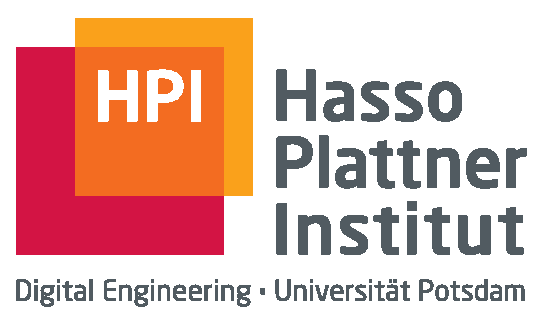
\includegraphics[width=0.2\textwidth]{hpi_logo_2017}\\
  \vspace{24pt}
  In-Memory Trajectory Analysis on Taxi Data
}
\subtitle{
  Seminar Trends and Concepts 3\\
  Summer Semester 2018
}

\numberofauthors{3}

\author{
  Marcel Jankrift\\
  Sebastian Kliem\\
  Toni Stachewicz\\[12pt]
  Supervisors:\\
  Dr. Matthias Uflacker, Keven Richly
}

\maketitle
\begin{abstract}
The taxi business is an extremely competitive market. Private ridesharing companies such as Uber or Lynx have grown tremendously in the last decade. In order to survive as a traditional taxi company, the drivers have to increase their profit even further. Therefore, we created an application, that analysis taxi data recorded over one day in the city of Shenzhen. We examine which taxis were the most profitable ones by calculating the distances and times driven with a passenger. From this information, we can draw specific recommendations, where to take passengers at a certain time, so that the profit can be maximized.
\end{abstract}


\keywords{Geospatial data, Trajectory analysis, Taxi data, In-Memory}

\section{Motivation}

\section{Data Sources}

The data we used is a freely available collection of GPS information of taxis. \footnote{\href{https://www-users.cs.umn.edu/~tianhe/BIGDATA/UrbanCPS/TaxiData/TaxiData}{https://www-users.cs.umn.edu/$\sim$tianhe/BIGDATA/UrbanCPS/TaxiData/TaxiData}} The dataset set has been collected over one day starting at 12 AM and 23:59 PM in the city of Shenzhen, China and the surrounding area. The data does not only contain the GPS location at a certain time, but also the current speed and the taxi's occupancy. The status of a driving taxi has been recorded in an average interval of 26.85 seconds or every 15 seconds in median. In total there are 14,728 trajectories traced resulting in almost 47 million records. The data comes in CSV-format which can be loaded into the SAP HANA database immediately. The total memory consumption without any further optimization (e.g. indices) of the Shenzhen data takes 541 MB.

\subsection{Data Cleansing}

\section{Application Prototype}

\subsection{System Architecture}

\subsection{Data Layouts}

\subsection{Optimizations}

\section{Benchmark Results}

\section{Future Work}

\section{Conclusion}

\section{References}
Generated by bibtex from your ~.bib file.  Run latex,
then bibtex, then latex twice (to resolve references)
to create the ~.bbl file.  Insert that ~.bbl file into
the .tex source file and comment out
the command \texttt{{\char'134}thebibliography}.

\end{document}
